A face rotation can be performed by taking advantage of the symmetric of the face, where both eyes are mirrored from the line that goes through the center point of the face and is aligned along the y-axis. This is done by extracting the eyes from the eye map and use the symmetric line to get the correct rotation angle.
\newline
REF!!!
The algorithm used to locate the eyes as circle object, is called Circular Hough Transform, CHT. The algorithm is mainly used because of its robustness at noisy areas, occlusion and varying illumination. There are no specific steps to implement the algorithm, therefore, a short description of the chosen steps is presented as follows.
\newline
\newline
The first step is to compute the accumulator array. The foreground pixels of high gradients are chosen to act as candidate pixels, they are allowed to cast "votes" in the accumulator array. The candidate pixels vote in a circle pattern around them with a fixed radius, see figure \ref{fig:CHT}
\newline
\begin{figure}[H]
\centering

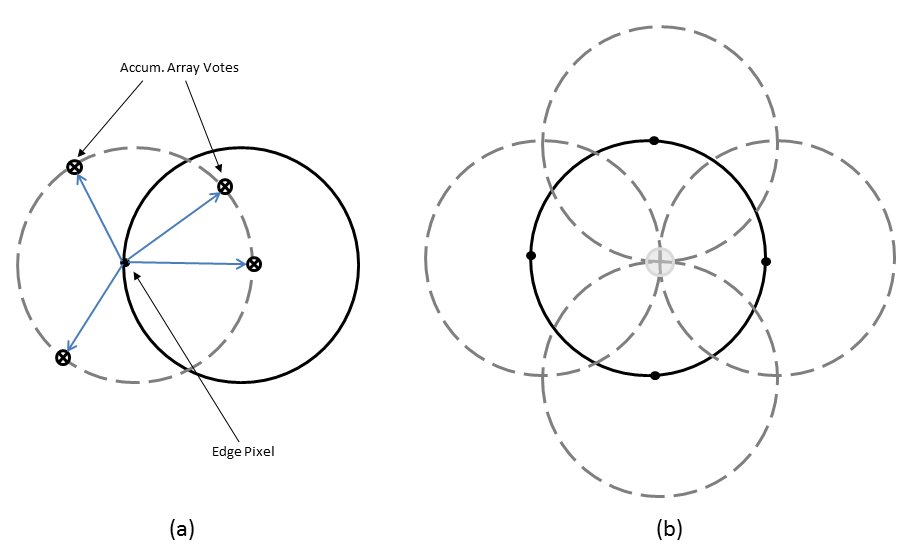
\includegraphics[scale=0.4]{img/fd/accarray.png}

\caption{CHT voting pattern to estimate the center of the circle.}
\label{fig:CHT}
\end{figure}
\indent 
The second step is to estimate the center. The position votes of candidate pixels belonging to an image circle tend to accumulate at the center of the circle. Therefore, the center of the circle is estimated by detecting the peaks in the accumulator array, where the votes are stored.

When the eyes are located and extracted, a rotation of the face can finally be performed.  The goal is to rotate the vector, that has its start point at the left eye and end point at the right eye, so that it is parallel with the x-axis. The rotation angle is estimated by the properties of the definition of the dot product operation.
